\chapter{User Manuals}
 All console programs can be shut down by the key combination \texttt{CTRL+C}. To test if a tool which provides data through D-Bus is working and sending the correct values, the Qt tool qdbusviewer can be used. The qdbusviewer can connect to the D-Bus interface provided by the daemons and display the data that flows through it.

 \section{Compilation}
  Before any of the programs can be used the programs need to be compiled. To do so you have to change into the topmost building directory (where all the application directories are located in). The directory listing should look similar to the one shown in listing \ref{lst:manual:compilation:directoryList}
  \begin{lstlisting}[frame=single,breaklines,basicstyle=\footnotesize,numbers=left,label=lst:manual:compilation:directoryList,captionpos=b,caption={Project directory list}]
CMakeLists.txt
common/
firmware/
gainData/
generatePosition/
obConfig/
pdAdmin/
showPos/
  \end{lstlisting}
  To compile all the daemons and applications now type the following two commands:
  \begin{verbatim}
   cmake .
   make
  \end{verbatim}
  \fbox{\textbf{ATTENTION}: After the cmake command is a dot and it belongs there.}\\
  If you want to enable debug flags of the applications you have to do the following:
  \begin{verbatim}
   cmake -DDEBUG=1 .
   make
  \end{verbatim}

  Only the firmware has to be compiled differently, but a pre compiled version of the current one is already in the directory. The firmware is also in need of a special c compiler for the arm CPU which needs to be installed on the system. To compile the firmware change into the \verb=firmware= directory and type:
  \begin{verbatim}
   make
  \end{verbatim}
  This will create a \verb=openbeacon.bin= file which is the firmware and can be flashed with the OpenBeacon Configurator (see section \ref{sec:manual:hardwareSimulator}). The file with no further code changes should have a file size of $24668$ byte if it differs then your compiler might have done something wrong and the firmware might not work with the hardware. So if you change the source of the firmware build it unchanged before changing it and then check if your size differs from the original.

  A set of pre build firmwares is available in the directory \verb=firmware/build/=, it contains at least the following files:
  \begin{lstlisting}[frame=single,breaklines,basicstyle=\footnotesize,numbers=left,label=lst:manual:compilation:prebuildFirmwaresList,captionpos=b,caption={Pre-build OpenBeacon USB firmwares}]
estimator-008-dld-01.bin
estimator-008.bin
  \end{lstlisting}
  Where the first is the one created for this project and the second one is the original one coming with the nodes.

 \section{OpenBeacon Configurator - Application}
 \label{sec:manual:OBConfigurator}
  The OpenBeacon Configurator is an easy to use graphical user interface which helps the user with the configuration and the flashing of the OpenBeacon nodes.
  \begin{staticFigure}
   \begin{center}
     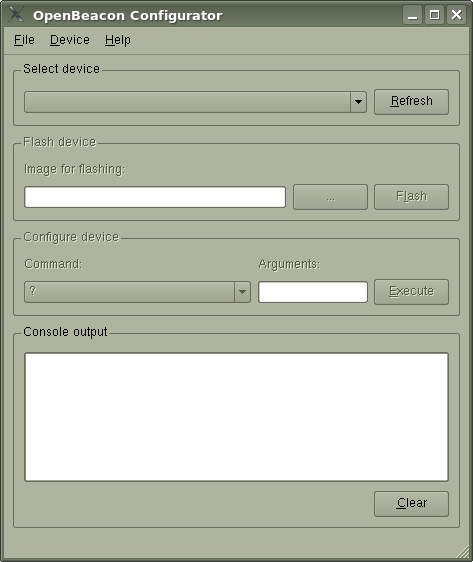
\includegraphics[scale=0.8]{images/UserManual/obConfig/mainWindow.png}
     \caption{The main window of the OpenBeacon Configurator}
     \label{fg:userManual:obConfig:mainWindow}
   \end{center}
  \end{staticFigure}

  \subsection{Pre requirements}
   To use the OpenBeacon Configurator a few things need to be done before.
   \begin{enumerate}
    \item The kernel must be capable of seeing the devices, therefore the following modules needs to be enabled:
     \begin{itemize}
      \item usbserial
      \item cdc-acm
     \end{itemize}
     If they do not exist they have to be enabled in the kernel. For further notes have a look into your kernel sources and the listings \ref{lst:kernelEnableACM} and \ref{lst:kernelEnableUSBSerial} (both located in the research chapter) to get a clue where to find them.
    \item Install the sam7 package provided by the OpenBeacon project. You can download it from here: \url{http://www.openpcd.org/dl/sam7utils-0.1.0-bm.tar.bz2}.
    \item While the cdc-adm module is just loaded the usbserial module needs to be loaded with certain parameters. With the following command the usbserial module gets told that it should be used for a specific product from a specific vendor:\\
    \verb% modprobe usbserial vendor=0x03eb product=0x6124%
   \end{enumerate}

  \subsection{Flashing a device}
  \label{sec:userManual:obConfig:flashingADevice}
   To flash a device, the prior system on it must be erased. To do so the following steps need to be performed:
   \begin{enumerate}
    \item Unplug the USB cable and insert the SAM-BA jumper (Pin 1+2)
    \item Attach the USB cable
    \item Wait ten seconds
    \item Unplug the USB cable
    \item Remove the SAM-BA jumper
    \item Attach the USB cable
    \item Wait several seconds to allow the device to be detected by Linux
   \end{enumerate}
   After that a ttyUSB device should show up in the device list.
   \begin{staticFigure}
    \begin{center}
     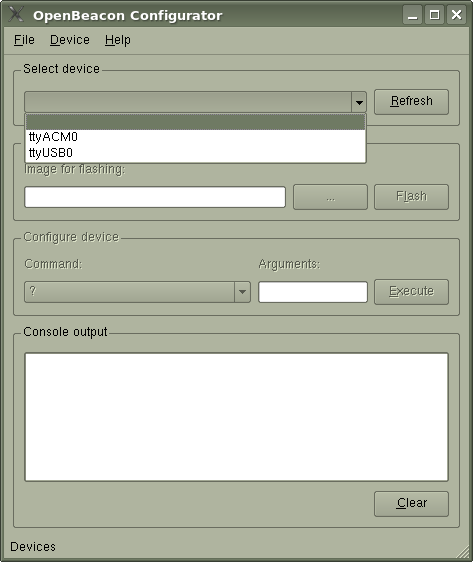
\includegraphics{images/UserManual/obConfig/mainWindow-deviceSelection.png}
     \caption{OpenBeacon Configurator with expanded device selection}
     \label{fg:userManual:obConfig:mainWindow-deviceSelection}
    \end{center}
   \end{staticFigure}
   Figure \ref{fg:userManual:obConfig:mainWindow-deviceSelection} shows that the OpenBeacon configurator has both devices available. For flashing select the ttyUSB device. After that the flash section will be available for editing and an image for flashing can be chosen. The button with the three dots opens a file dialog from which a suitable file can be chosen. After selection the screen should be look like in figure \ref{fg:userManual:obConfig:mainWindow-beforeFlashing}.
   \begin{staticFigure}
    \begin{center}
     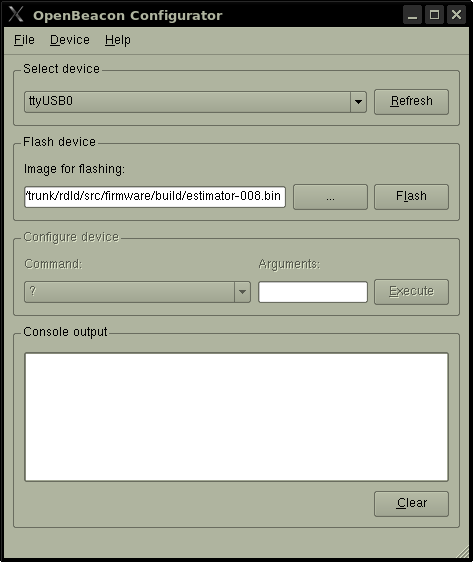
\includegraphics{images/UserManual/obConfig/mainWindow-beforeFlashing.png}
     \caption{OpenBeacon Configurator with selected image}
     \label{fg:userManual:obConfig:mainWindow-beforeFlashing}
    \end{center}
   \end{staticFigure}
   When the selection of the image is finished the flashing can be started by pressing the Flash button. The flashing then will interrupt the application until the whole flashing is done. After the flashing the main window should look like in figure \ref{fg:userManual:obConfig:mainWindow-afterFlashing}.
   \begin{staticFigure}
    \begin{center}
     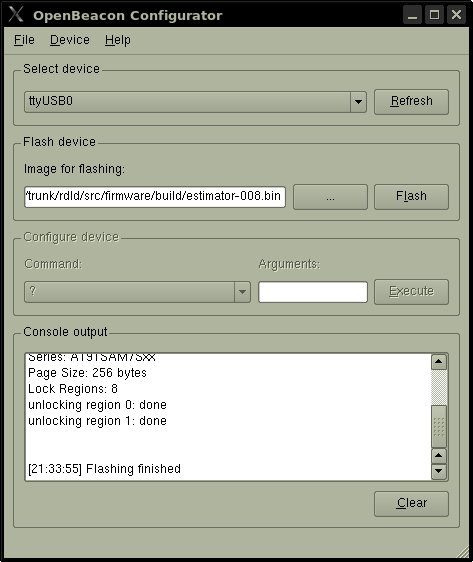
\includegraphics{images/UserManual/obConfig/mainWindow-afterFlashing.png}
     \caption{OpenBeacon Configurator after flashing}
     \label{fg:userManual:obConfig:mainWindow-afterFlashing}
    \end{center}
   \end{staticFigure}

  \subsection{Configuring a device}
   To configure a device select it from the ``Select device'' pull down menu. An already flashed device is one of the ttyACM ones; if there are only ttyUSB devices then one of the devices needs to be flashed before (see \ref{sec:userManual:obConfig:flashingADevice}). If the correct device is selected the screen looks similar to the following:
   \begin{staticFigure}
    \begin{center}
     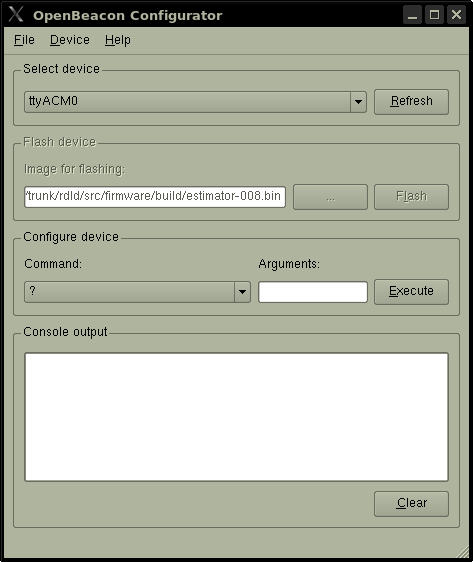
\includegraphics{images/UserManual/obConfig/mainWindow-beforeCommandExe.png}
     \caption{OpenBeacon Configurator before command execution}
     \label{fg:userManual:obConfig:mainWindow-beforeCommandExe}
    \end{center}
   \end{staticFigure}

   The first action we perform is a command without arguments, the ``?'' command, which will display the help screen of the firmware. Figure \ref{fg:userManual:obConfig:mainWindow-afterCommandExe} shows the main window with an executed ``?'' command.
   \begin{staticFigure}
    \begin{center}
     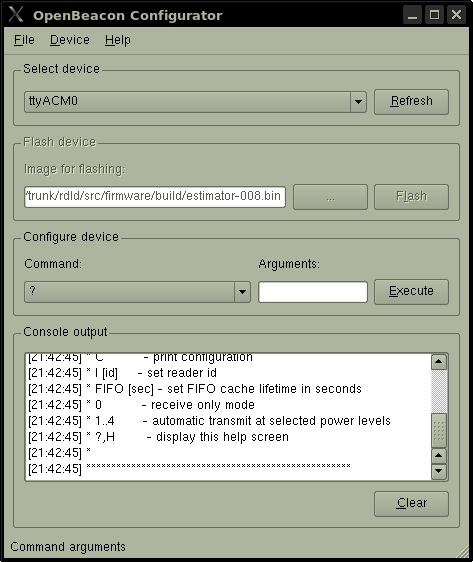
\includegraphics{images/UserManual/obConfig/mainWindow-afterCommandExe.png}
     \caption{OpenBeacon Configurator after command execution}
     \label{fg:userManual:obConfig:mainWindow-afterCommandExe}
    \end{center}
   \end{staticFigure}

   The second action is a command with an argument. The ``I'' command which changes the current id of the OpenBeacon node, it also requires a number as argument, which defines the new id of the node. Figure \ref{fg:userManual:obConfig:mainWindow-afterCommandWithArg} shows the execution of this command with the argument ``4''.
   \begin{staticFigure}
    \begin{center}
     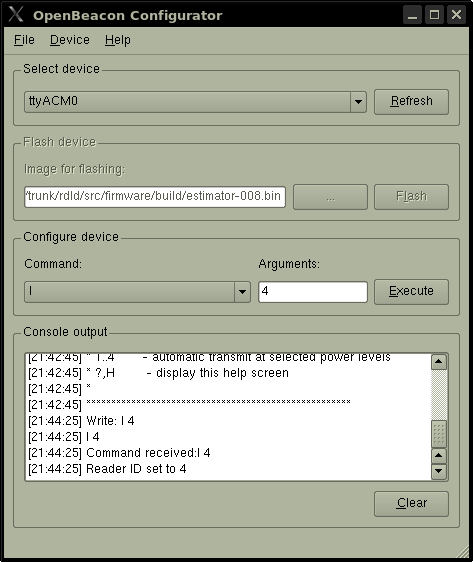
\includegraphics{images/UserManual/obConfig/mainWindow-afterCommandWithArg.png}
     \caption{OpenBeacon Configurator after command execution with an argument}
     \label{fg:userManual:obConfig:mainWindow-afterCommandWithArg}
    \end{center}
   \end{staticFigure}

  \subsection{Personalise the configurator}
   To personalise the ``OpenBeacon Configurator'' it provides a preference dialog. Figure \ref{fg:userManual:obConfig:preferenceInitial} shows the initial preference dialog. It is filled with the default values in this case only the help command.
   \begin{staticFigure}
    \begin{center}
     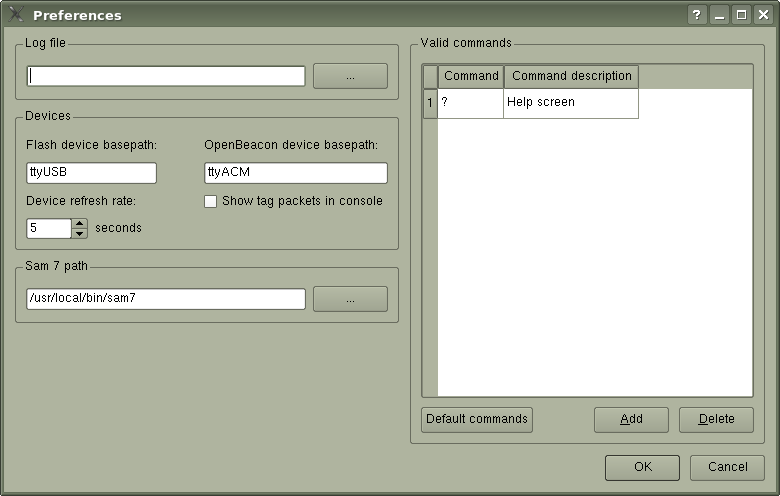
\includegraphics[scale=0.7]{images/UserManual/obConfig/preferenceWindow-initial.png}
     \caption{OpenBeacon Configurator preference dialog}
     \label{fg:userManual:obConfig:preferenceInitial}
    \end{center}
   \end{staticFigure}
   On the left part of the preference dialog are path and GUI specific preferences. The log file path defines the file where the logging should be redirected instead of the console. The sam7 path is the path to the sam7 binary. And the device specific parameter defines the base names of the different devices, the update interval in which the device pull down should be refreshed and a check box with whom the periodic information about the packet loss from the tags can be suppressed.

   The right part of the dialog contains the commands that should be available for the ``OpenBeacon Configurator''. The ``Default Commands'' button opens a dialog (see figure \ref{fg:userManual:obConfig:preferenceDefaultCommands}) where you can choose which command collection should \textbf{replace} the current list.
   \begin{staticFigure}
    \begin{center}
     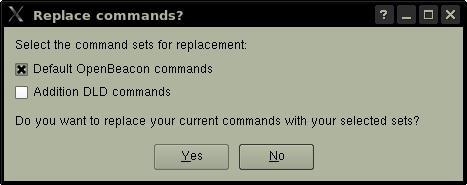
\includegraphics{images/UserManual/obConfig/preferenceWindow-defaultCommands.png}
     \caption{Default Commands Dialog from the preferences}
     \label{fg:userManual:obConfig:preferenceDefaultCommands}
    \end{center}
   \end{staticFigure}
   To add a single command simply click the ``Add'' button and an empty line will be inserted at the top of the table (see figure \ref{fg:userManual:obConfig:preferenceAddCommand}).
   \begin{staticFigure}
    \begin{center}
     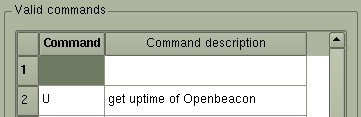
\includegraphics{images/UserManual/obConfig/preferenceWindow-cmdAdd.png}
     \caption{Empty entry added to command list}
     \label{fg:userManual:obConfig:preferenceAddCommand}
    \end{center}
   \end{staticFigure}
   After the empty line is added it can be edited by double clicking the cell (see figure \ref{fg:userManual:obConfig:preferenceAddCommandEdited}). Both fields need to be filled.
   \begin{staticFigure}
    \begin{center}
     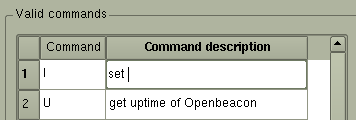
\includegraphics{images/UserManual/obConfig/preferenceWindow-cmdAddEdit.png}
     \caption{Recently added entry will be changed}
     \label{fg:userManual:obConfig:preferenceAddCommandEdited}
    \end{center}
   \end{staticFigure}

   To remove a command simply select a cell from the command table and click the ``Delete'' button, it will delete the whole entry.

   If the preference dialog is closed through the ``OK'' button all changes will be stored permanently.

 \section{Data gain - Daemon}
  The data gain daemon gains the strength information from the hardware devices and provides them to other applications.

  \subsection{Configuration of the daemon}
   The configuration file is located at the following position: \texttt{~/.config/DLD/Gain data daemon.conf}. Right now it has only one configuration parameter.
   \begin{table}[h]
    \centering
    \begin{tabular}{|l|l|l|}
     \hline
      \textbf{Parameter name}		& \textbf{Description}			& \textbf{Possible values} (if applicable)\\
     \hline
      \multirow{4}*{usedDeviceStrategy}	& describes the hardware 		& \textbf{Hardware Simulator}:\\
					& strategy that will be used		& DLDSimulateStrategy\\
					& 					& \textbf{OpenBeacon Hardware}:\\
					&					& OpenBeaconUSBStrategy\\
     \hline
    \end{tabular}
    \caption{Configuration values for the configuration file}
    \label{tab:manual:gainDaemon:configValues}
   \end{table}
   The \textit{usedDeviceStrategy} parameter is located in the General section of the configuration file.
  \subsection{Command line parameter}
   \begin{table}[h]
    \centering
    \begin{tabular}{|l|l|c|l|}
     \hline
      \textbf{Parameter}	& \textbf{Value}	& \textbf{Possible}	& \textbf{Description}\\
      \textbf{name}		&			& \textbf{values}	& \\
     \hline
      \multirow{8}*{-v}		& value			&			& The level of verbosity\\
				&			& 0			& \textbf{Quiet} mode - print nothing\\
				&			& 1			& \textbf{Error} mode - print errors\\
				&			&			& (default)\\
				&			& 2			& \textbf{Info} mode - adds info\\
				&			&			& messages\\
				&			& 3			& \textbf{Debug} mode - adds debug\\
				&			&			& messages\\
     \hline
      \multirow{3}*{-l}		& logFile		&			& File name where the\\
				&			&			& messages should be logged\\
				&			&			& to instead of console\\
     \hline
      \multirow{3}*{-s}		& strategy		& OpenBeaconUSBStrategy	& Use OpenBeacon USB\\
				&			&			& strategy\\
				&			& DLDSimulateStrategy	& Use Hardware Simulator\\
     \hline
    \end{tabular}
    \caption{Command line parameters for the data gain daemon}
    \label{tab:manual:gainDaemon:commandLineParameter}
   \end{table}

  \subsection{Configuration and start up examples}
   \subsubsection*{With configuration and no command line parameters}
    If the configuration file contains the same as listing \ref{lst:manual:gainData:exampleConfiguration} shows, the daemon will start the hardware simulator.
    \begin{lstlisting}[frame=single,breaklines,basicstyle=\footnotesize,numbers=left,label=lst:manual:gainData:exampleConfiguration,captionpos=b,caption={Example Configuration file for the data gain daemon}]
[General]
usedDeviceStrategy=DLDSimulateStrategy
    \end{lstlisting}
    After the configuration is done the data gain daemon can be simply started with the following command:
    \begin{verbatim}
     gainData
    \end{verbatim}
    As soon as the daemon is ready it should display the hardware simulator. For further instructions look at the user manual for the hardware simulator in section \ref{sec:manual:hardwareSimulator}.

   \subsubsection*{Only command line parameters}
    If no configuration file is available the used strategy will be chosen by command line or if even this is not given the default value (\texttt{OpenBeaconUSBStrategy}) will be used. To start the gain data daemon showing debug messages to the console and use the ``Hardware Simulator'' strategy, the command is the following:
    \begin{verbatim}
     gainData -v 3 -s DLDSimulateStrategy
    \end{verbatim}
    The selected strategy will be stored in the configuration file as soon as the daemon will be shut down.

   \subsubsection*{No configuration and no command line parameters}
    If the data gain daemon is started without command line parameters nor an existing configuration file is existent, the daemon only shows error messages printed to the console and uses the \texttt{OpenBeaconUSBStrategy} as the default hardware strategy. The command for this will be:
    \begin{verbatim}
     gainData
    \end{verbatim}
    After the gain data daemon is closed the configuration file will be created and the default strategy will be stored.

   \subsubsection{Configuration of the ``OpenBeacon USB Strategy''}
    The configuration file is located at the following position:\\
    \indent\texttt{~/.config/DLD/obUSBStrategy.conf}.\\
    \begin{table}[h]
     \centering
     \begin{tabular}{|l|l|l|}
      \hline
       \multirow{2}*{Parameter name}	& \textbf{Description}			& \textbf{Possible values}\\
					& 					& (if applicable)\\
      \hline
       \multirow{3}*{maxPackagesOnOB}	& Maximum amount of packages		& 1-30\\
					& an OB device stores per sec		& \\
					& (FIFO)				& \\
      \hline
       \multirow{1}*{id}		& The nodes id				& \\
      \hline
       \multirow{1}*{x}			& The X Coordination of the node	& \\
      \hline
       \multirow{1}*{y}			& The Y Coordination of the node	& \\
      \hline
       \multirow{1}*{z}			& The Z Coordination of the node	& \\
      \hline
     \end{tabular}
     \caption{Configuration values for the OpenBeacon USB Strategy}
     \label{tab:manual:gainDaemon:configOBUSBStrategy}
    \end{table}
    The \textit{maxPackagesOnOB} parameter is located in the General section of the configuration file. The other parameters, \textit{id}, \textit{x}, \textit{y}, and \textit{z}, are located in a section called OpenBeacon-N, where the N is the number of the configured node. The numbers have to start from 0 and every following node has to have an increased number of its predecessor.

   \subsubsection{Example configuration for the ``OpenBeacon USB Strategy''}
    Listing \ref{lst:manual:gainData:exampleConfigurationOBUSBStrategy} shows a configuration example for 3 nodes, who all have a maximum of 30 packages to loose per second.
    \begin{lstlisting}[frame=single,breaklines,basicstyle=\footnotesize,numbers=left,label=lst:manual:gainData:exampleConfigurationOBUSBStrategy,captionpos=b,caption={Example Configuration file for the OpenBeacon USB Strategy}]
[General]
maxPackagesOnOB=30

[OpenBeacon-0]
id=5
x=0
y=0
z=0

[OpenBeacon-1]
id=24
x=-3.5
y=0
z=0

[OpenBeacon-2]
id=2
x=0
y=15.5
z=0
    \end{lstlisting}
  The higher the \verb=maxPackagesOnOB= (the OpenBeacon FIFO value) value the higher the accuracy of the tags will be.

 \section{Generate position - Daemon}
  The generate position daemon calculates the position of a tag on base of the strength values the data gain daemon is providing. Therefore it only works after the data gain daemon is configured and runs.

  \subsection{Configuration of the daemon}
   Right now the generate position daemon has no configuration values. At the current state the only available strategy is a two dimensional location detection. But later on it might be possible that a three dimensional location detection can be implemented.

  \subsection{Command line parameter}
   \begin{table}[h]
    \centering
    \begin{tabular}{|l|l|c|l|}
     \hline
      \textbf{Parameter}	& \textbf{Value}	& \textbf{Possible}	& \textbf{Description}\\
      \textbf{name}		&			& \textbf{values}	& \\
     \hline
      \multirow{8}*{-v}		& value			&			& The level of verbosity\\
				&			& 0			& \textbf{Quiet} mode - print nothing\\
				&			& 1			& \textbf{Error} mode - print errors\\
				&			&			& (default)\\
				&			& 2			& \textbf{Info} mode - adds info\\
				&			&			& messages\\
				&			& 3			& \textbf{Debug} mode - adds debug\\
				&			&			& messages\\
     \hline
      \multirow{3}*{-l}		& logFile		&			& File name where the\\
				&			&			& messages should be logged\\
				&			&			& to instead of console\\
     \hline
    \end{tabular}
    \caption{Command line parameters for the generate position daemon}
    \label{tab:manual:genPosDaemon:commandLineParameter}
   \end{table}

  \subsection{Example start}
   \begin{lstlisting}[frame=single,breaklines,basicstyle=\footnotesize,numbers=left,label=lst:manual:genPosDaemon:exampleStart1,captionpos=b,caption={Example start of the generate position daemon}]
genPos
   \end{lstlisting}
   \begin{lstlisting}[frame=single,breaklines,basicstyle=\footnotesize,numbers=left,label=lst:manual:genPosDaemon:exampleStart2,captionpos=b,caption={Example start of the generate position daemon with higher verbosity}]
genPos -v 3
   \end{lstlisting}
   Listing \ref{lst:manual:genPosDaemon:exampleStart1} shows a general start up of the client and listing \ref{lst:manual:genPosDaemon:exampleStart1} shows an example start but with a higher verbosity level. The higher verbosity level will enable a lot of messages that will be sent to the console.

 \section{Administrate person data - Application}
  The person data administration application is used to add persons to the persons database. As pre requirement a database needs to be created. See section \ref{sec:implementation:pdAdmin} for further information how to create the database.

  After the start of the application it presents itself with the following screen:
  \begin{staticFigure}
   \begin{center}
     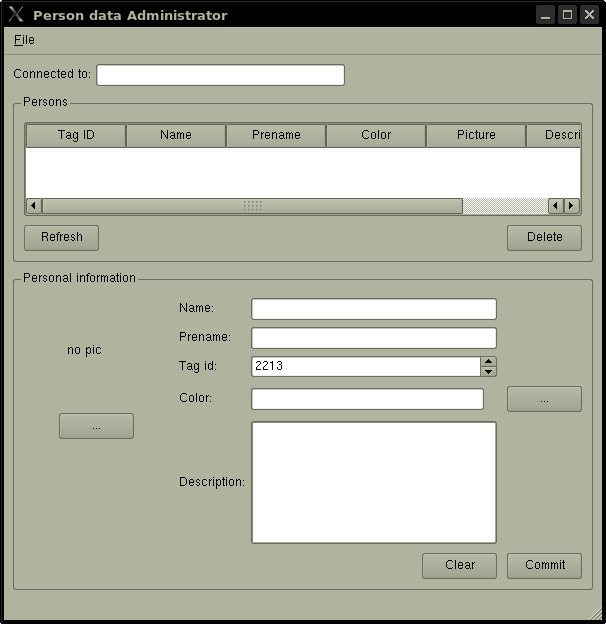
\includegraphics[scale=0.5]{images/UserManual/pdAdmin/main.png}
     \caption{The main window of the Administrate person data application}
     \label{fg:userManual:pdAdmin:mainWindow}
   \end{center}
  \end{staticFigure}

  Before any of the functionality is useful, the ``Person Data Administrator'' needs to be connected to the database. To connect to the database press the key combination \texttt{CTRL+C} or use the menu like shown in figure \ref{fg:userManual:pdAdmin:menu}.
  \begin{staticFigure}
   \begin{center}
     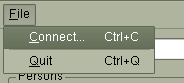
\includegraphics{images/UserManual/pdAdmin/menu.png}
     \caption{Select connect from file menu}
     \label{fg:userManual:pdAdmin:menu}
   \end{center}
  \end{staticFigure}

  As soon as connect was selected a dialog for the connection will appear (see figure \ref{fg:userManual:pdAdmin:connectDialog}).
  \begin{figure}[h]
   \centering
     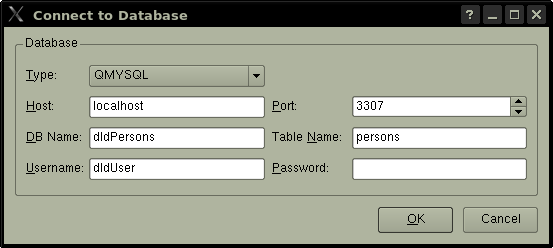
\includegraphics{images/UserManual/pdAdmin/connectDialog.png}
     \caption{Database connection dialog}
     \label{fg:userManual:pdAdmin:connectDialog}
  \end{figure}
  The dialog will be refilled by the values that were used in an old session if this is the first time the ``Person Data Administrator'' is launched all fields will be empty. After the connection was successful the contents of the main screen will change. The topmost field shows the name database, the application is connected to.
  \begin{staticFigure}
   \begin{center}
     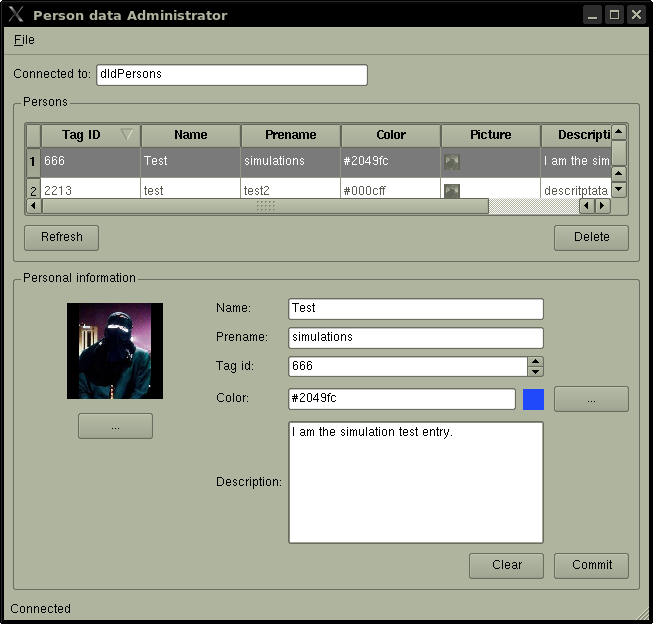
\includegraphics[scale=0.8]{images/UserManual/pdAdmin/mainSelectedEntry.png}
     \caption{Main screen with selected entry}
     \label{fg:userManual:pdAdmin:mainSelectedEntry}
   \end{center}
  \end{staticFigure}
  Below is a list of the entries that are stored in the database and the lowest group box (Personal Information) stores a detailed view of the selected entry. If an entry is selected the data can be changed in this group box as well. To store the changes the ``Commit'' button needs to be pressed.

  To create a new entry the Personal Information group box needs to be filled with new data, the tag id will be used as the key value, therefore only the tag id must be different from the other entries. To clear all fields (i.e. you want to create a new entry) press the clear button. This will not delete an entry it just clears all the fields. The ``\dots'' button right next to the colour field will open a dialog (see figure \ref{fg:userManual:pdAdmin:selectColor}) which allows the selection of the colour.
  \begin{staticFigure}
   \begin{center}
     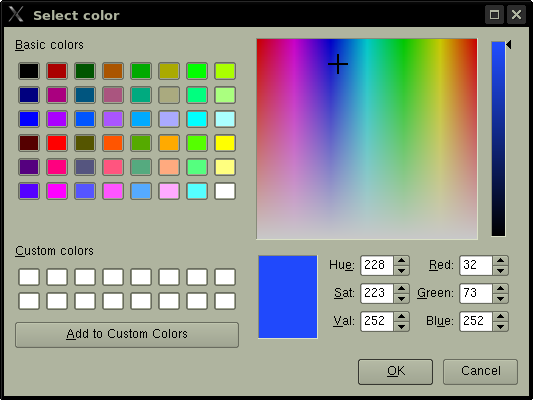
\includegraphics{images/UserManual/pdAdmin/selectColorDialog.png}
     \caption{Colour selection}
     \label{fg:userManual:pdAdmin:selectColor}
   \end{center}
  \end{staticFigure}
  The ``\dots'' button below the picture on the other hand opens a dialog (see figure \ref{fg:userManual:pdAdmin:selectPicture}) to select an image which will represent the person.
  \begin{staticFigure}
   \begin{center}
     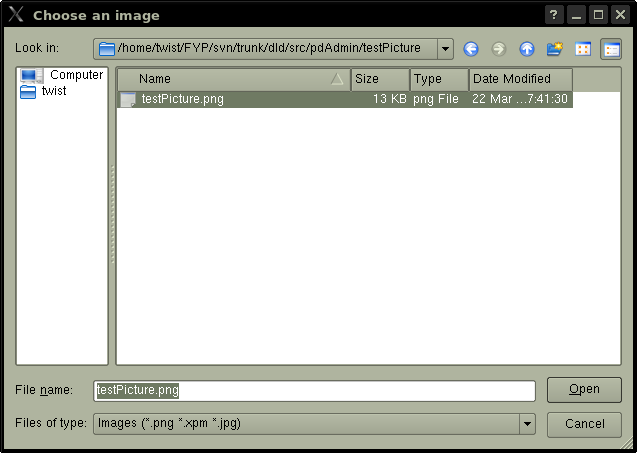
\includegraphics[scale=0.8]{images/UserManual/pdAdmin/choosePictureDialog.png}
     \caption{Picture selection}
     \label{fg:userManual:pdAdmin:selectPicture}
   \end{center}
  \end{staticFigure}

  If an entry should be deleted the entry needs to be selected and then a click on the delete button will remove the entry permanently from the database.

 \section{Show position - Application}
  Right after the ``Show position'' application is launched it presents itself like shown in figure \ref{fg:userManual:showPos:mainWindow}.
  \begin{staticFigure}
   \begin{center}
     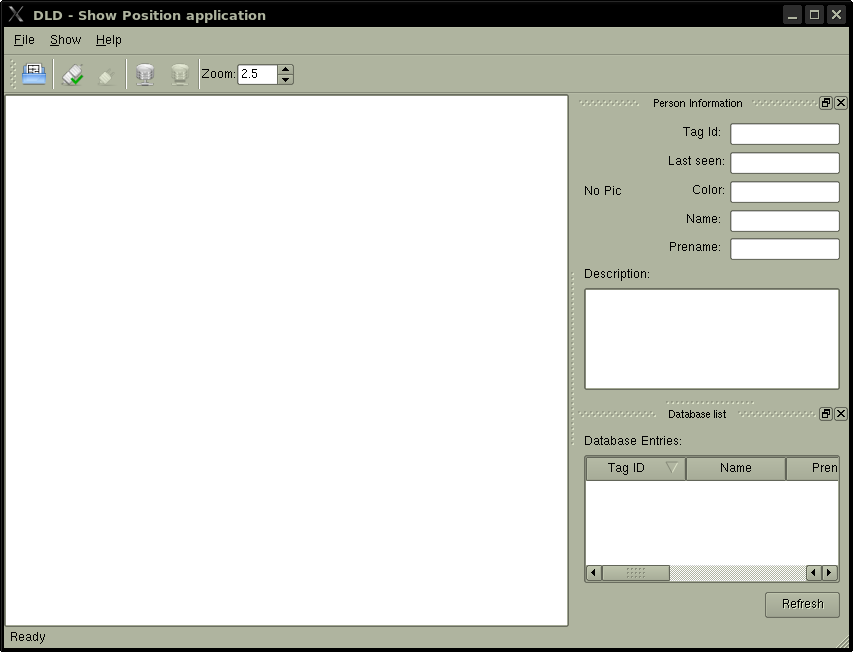
\includegraphics[scale=0.6]{images/UserManual/showPos/main.png}
     \caption{Main window of show position application}
     \label{fg:userManual:showPos:mainWindow}
   \end{center}
  \end{staticFigure}
  The centre widget will be used to display the map and the tags. On the right side are two dock widgets, one shows the person information of the current selected tag and below is a widget which displays the entries that are loaded from the database.
  
  At first the ``show position'' application should be connected to the database (if it is available), this action can be performed through three different ways. the first one is to click the ``Connect to Database'' toolbar button 
\includegraphics[scale=0.15]{images/UserManual/showPos/icons/db-connect.png}, the menu: \texttt{File->Connect to database}, or the key combination \texttt{CTRL+S}. After requesting the connection it will open the same database connection dialog like it was used in the ``Administrate person data'' application (see figure \ref{fg:userManual:pdAdmin:connectDialog}). After the connection is built up the ``Database entries'' widget contains a list of the entries (see figure \ref{fg:userManual:showPos:databaseEntriesWidget}).
  \begin{staticFigure}
   \begin{center}
     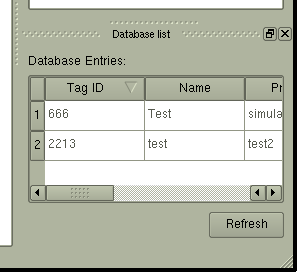
\includegraphics[scale=0.6]{images/UserManual/showPos/main-connected2DB.png}
     \caption{Database entries widget filled with a few entries}
     \label{fg:userManual:showPos:databaseEntriesWidget}
   \end{center}
  \end{staticFigure}

  After the connection to the person information database is built up the ``show position'' application needs to be connected to the ``generate position daemon''. To perform this action there are again three ways to do it, a button 
\includegraphics[scale=0.15]{images/UserManual/showPos/icons/connect.png} at the toolbar, the menu: \texttt{File->Connect to Generate Position} or the key short cut \texttt{CTRL+C}. This action will pop up a connection dialog where you have the choice how you want to connect to the ``generate position daemon'', through D-Bus or through SSL. SSL is not working at the moment because it was not implemented, so the only working choice is the D-Bus connection.
  \begin{staticFigure}
   \begin{center}
     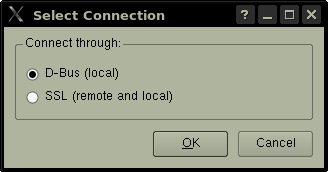
\includegraphics{images/UserManual/showPos/connect2GenPos.png}
     \caption{Connect to Generate position Dialog}
     \label{fg:userManual:showPos:connect2GenPos}
   \end{center}
  \end{staticFigure}

  Right after the connection to the generate position daemon is built up, the main screen will show a coordination system and if some tags are near the nodes, they will show up as well. The following figure (\ref{fg:userManual:showPos:mainWindowConnectedOneTag}) shows this state with a blue tag.

  \begin{staticFigure}
   \begin{center}
     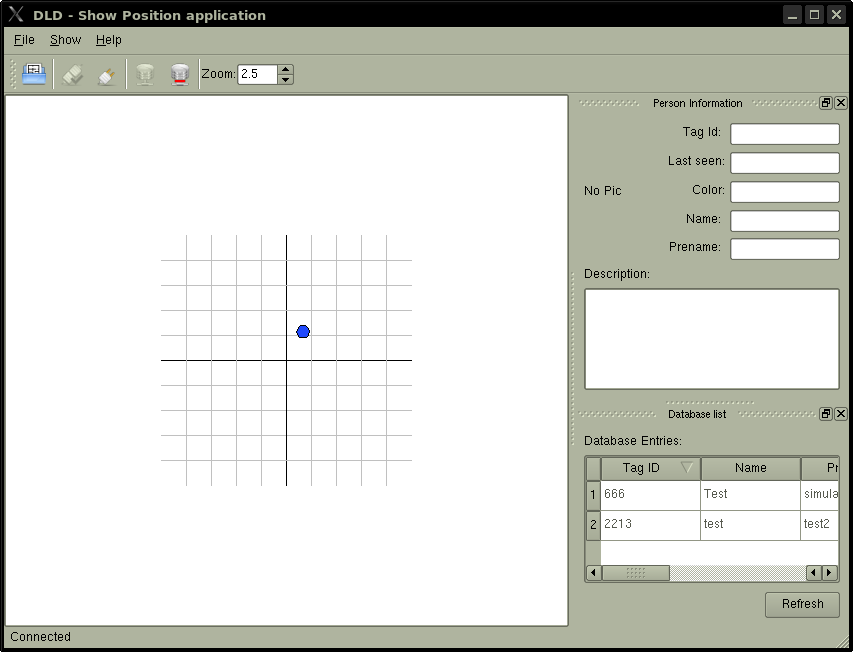
\includegraphics[scale=0.55]{images/UserManual/showPos/afterConnection2GenPos-Tag.png}
     \caption{Main window with connections build up and a visible tag}
     \label{fg:userManual:showPos:mainWindowConnectedOneTag}
   \end{center}
  \end{staticFigure}

  If the mouse will be moved over the blue tag, the person information that is stored in the database will be displayed in the person information widget as well as on a widget that appears right next to the mouse cursor. Figure \ref{fg:userManual:showPos:mouseOverWidget} shows this widget with the entry for tag id 666.

  \begin{staticFigure}
   \begin{center}
     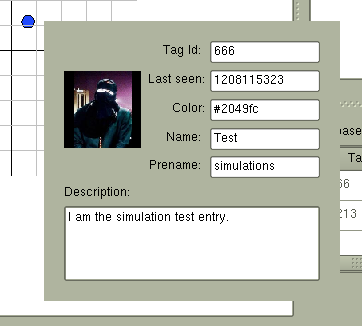
\includegraphics{images/UserManual/showPos/tagOnMouseOver.png}
     \caption{Widget that appears on mouse over}
     \label{fg:userManual:showPos:mouseOverWidget}
   \end{center}
  \end{staticFigure}

  To show or hide the widgets the check boxes in the \texttt{Show} menu can be selected or unselected.
 \section{Hardware Simulator - Application}
 \label{sec:manual:hardwareSimulator}
  The hardware simulator is launched by the data gain daemon. It will open a user interface that emulates the existence of three nodes and the strengths each of them is receiving. In addition it shows the current data in a graphical representation. Figure \ref{fg:manual:hardwareSimulator:mainScreen} shows the main screen of the hardware simulator. The whole simulator consists of this one screen.
  \begin{figure}[h]
   \centering
   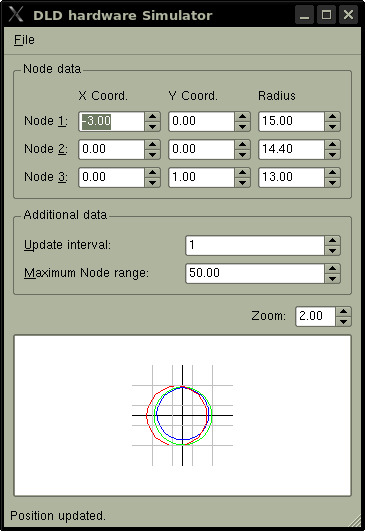
\includegraphics[scale=0.5]{images/UserManual/hwSim/mainScreen.png}
   \caption{hardware simulator main screen}
   \label{fg:manual:hardwareSimulator:mainScreen}
  \end{figure}
  The upper group box contains the coordinations and the strength data (radius) of nodes. The box below the coordinates contains general information. The update interval is the time (in seconds) the data nodes emit the data about their radii. The ``Maximum Node range'' is the length of one axis in one direction, the change of this value will take effect after the restart of the application. The lowest widget displays the different radii of the nodes (red for the first node, green for the second one and blue for the third node). Through the zoom value the view can be enlarged or shrunken.

  The hardware simulator can be closed by clicking \texttt{File -> Quit} or pressing the key combination \texttt{CTRL+Q}, this will also close the data gain daemon.
